\documentclass[a4paper, 12pt]{article}

\newcommand{\templates}{../../template}
\usepackage[a4paper, margin=2.5cm]{geometry}

\usepackage{enumitem}
\setlist[itemize]{noitemsep}
\setlist[enumerate]{noitemsep}

\let\oldpar\paragraph
\renewcommand{\paragraph}[1]{\oldpar{#1\\}\noindent}
\usepackage{graphicx}
\usepackage{hyperref}
\usepackage{makecell}

\newcommand{\settitolo}[1]{\newcommand{\titolo}{#1\\}}
\newcommand{\setprogetto}[1]{\newcommand{\progetto}{#1\\}}
\newcommand{\setcommittenti}[1]{\newcommand{\committenti}{#1\\}}
\newcommand{\setredattori}[1]{\newcommand{\redattori}{#1\\}}
\newcommand{\setrevisori}[1]{\newcommand{\revisori}{#1\\}}
\newcommand{\setresponsabili}[1]{\newcommand{\responsabili}{#1\\}}
\newcommand{\setversione}[1]{
	\ifdefined\versione\renewcommand{\versione}{#1\\}
	\else\newcommand{\versione}{#1\\}\fi
}
\newcommand{\setdestuso}[1]{\newcommand{\uso}{#1\\}}
\newcommand{\setdescrizione}[1]{\newcommand{\descrizione}{#1\\}}

\newcommand{\makefrontpage}{
	\begin{titlepage}
		\begin{center}

		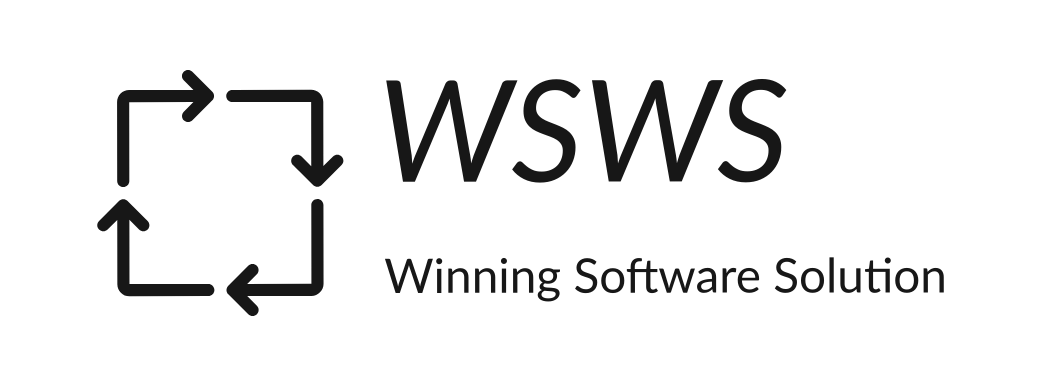
\includegraphics[width=0.4\textwidth]{../../template/WSWS-logos_transparent_crop}\\

		{\Large Winning Software Solution}\\[6pt]
		\href{mailto://winningsoftwaresolution@gmail.com}{winningsoftwaresolution@gmail.com}\\
		
		\ifdefined\progetto
		\vspace{1cm}
		{\Large\progetto}
		{\large\committenti}
		\else\fi
		
		\vspace{1.5cm}
		{\LARGE\titolo}
		
		\vfill
		
		\begin{tabular}{r | l}
		\multicolumn{2}{c}{\textit{Informazioni}}\\
		\hline
		
		\ifdefined\redattori
			\textit{Redattori} &
			\makecell[l]{\redattori}\\
		\else\fi
		\ifdefined\revisori
			\textit{Revisori} &
			\makecell[l]{\revisori}\\
		\else\fi
		\ifdefined\responsabili
			\textit{Respondabili} &
			\makecell[l]{\responsabili}\\
		\else\fi
		
		\ifdefined\versione
			\textit{Versione} & \versione
		\else\fi
		
		\textit{Uso} & \uso
		
		\end{tabular}
		
		\vspace{2cm}
		
		\ifdefined\descrizione
		Descrizione
		\vspace{6pt}
		\hrule
		\descrizione
		\else\fi
		\end{center}
	\end{titlepage}
}
\usepackage{hyperref}
\usepackage{array}
\usepackage{tabularx}

\def\vers#1-#2-#3-#4-#5\\{#1&#2&#3&#4&#5\\\hline}

\newcommand{\addversione}[5]{
	\ifdefined\versioni
		\let\old\versioni
		\renewcommand{\versioni}{#1&#2&#3&#4&#5\\\hline\old}
	\else
		\newcommand{\versioni}{#1&#2&#3&#4&#5\\\hline}
	\fi
}

\newcommand{\setversioni}[1]{\newcommand{\versioni}{#1}}

\newcommand{\makeversioni}{
	\begin{center}
		\begin{tabularx}{\textwidth}{|c|c|c|c|X|}
		\hline
		\textbf{Versione} & \textbf{Data} & \textbf{Persona} & \textbf{Attivtà} & \textbf{Descrizione} \\
		\hline
		\versioni
		\end{tabularx}
	\end{center}
	\clearpage
}
\usepackage{hyperref}
\usepackage{graphicx}
\usepackage{placeins}
\settitolo{Manuale Acquirente Shop Chain}
\setredattori{WinningSoftwareSolution}
\setdestuso{esterno}
\setdescrizione{
Manuale acquirente.
}

\begin{document}

\makefrontpage
\tableofcontents
\newpage

\section{Introduzione}
Attraverso l'utilizzo della blockchain \textit{Polygon}, Shop Chain fornisce un sistema decentralizzato per il pagamento di prodotti in MATIC. Utilizzando Shop Chain è possibile effettuare una qualsiasi attività di compravendita in maniera sicura per entrambi gli attori dello scambio. L'acquirente che desidera acquistare un prodotto da un venditore in un e-commerce potrà effettuare il suo pagamento in MATIC, ovvero il token nativo della blockchain \textit{Polygon}. Il venditore non può disporre immediatamente del saldo ricevuto poiché sarà bloccato fino alla ricezione del pacco, momento nel quale l'acquirente può sbloccare i fondi attraverso la scannerizzazione di un codice QR presente sulla scatola.\\
Il presente documento ha la funzione di descrivere in dettaglio la procedura da seguire per l'acquirente per il corretto acquisto di un item e successivo ritiro e sblocco fondi attraverso il servizio Shop Chain.

\section{Configurazione wallet}
\subsection{Wallet Metamask}
Per poter effettuare il pagamento sarà necessario l'utilizzo di un wallet Metamask. Visitare \href{https://www.metamask.io}{metamask.io} per maggiori informazioni.
\subsubsection{Configurazione}
\label{sec:network}
Se il network Polygon non è gia stato inserito nel proprio wallet Metamask, procedere con la lettura del seguente paragrafo.
Per l'inserimento e la configurazione del network Polygon nel proprio wallet Metamask è necessario utilizzare i seguenti dati:
\begin{itemize}
\item Network Name: \textbf{Matic Mainnet};
\item New RPC Url: \textbf{https://rpc-mainnet.maticvigil.com/};
\item ChainID: \textbf{137};
\item Currency Simbol: \textbf{MATIC};
\item Block Explorer URL: \textbf{https://explorer.matic.network/}.
\end{itemize}
Una volta inseriti i dati e aggiunto il network, selezionare il network prima di procedere con il pagamento.

\subsubsection{Collegamento a Shop Chain}
Per poter eseguire il pagamento è necessario collegare il proprio wallet Metamask a Shop Chain. Una volta reindirizzati sulla landing page di Shop Chain, se non si ha già collegato in precedenza il proprio wallet:
\begin {itemize}
\item selezionare "Connect Wallet" all'apertura del pop-up (Fig. 1);
\item approvare il collegamento dal proprio wallet Metamask.
\end{itemize}

\FloatBarrier
\begin{figure}[!h]
\centering
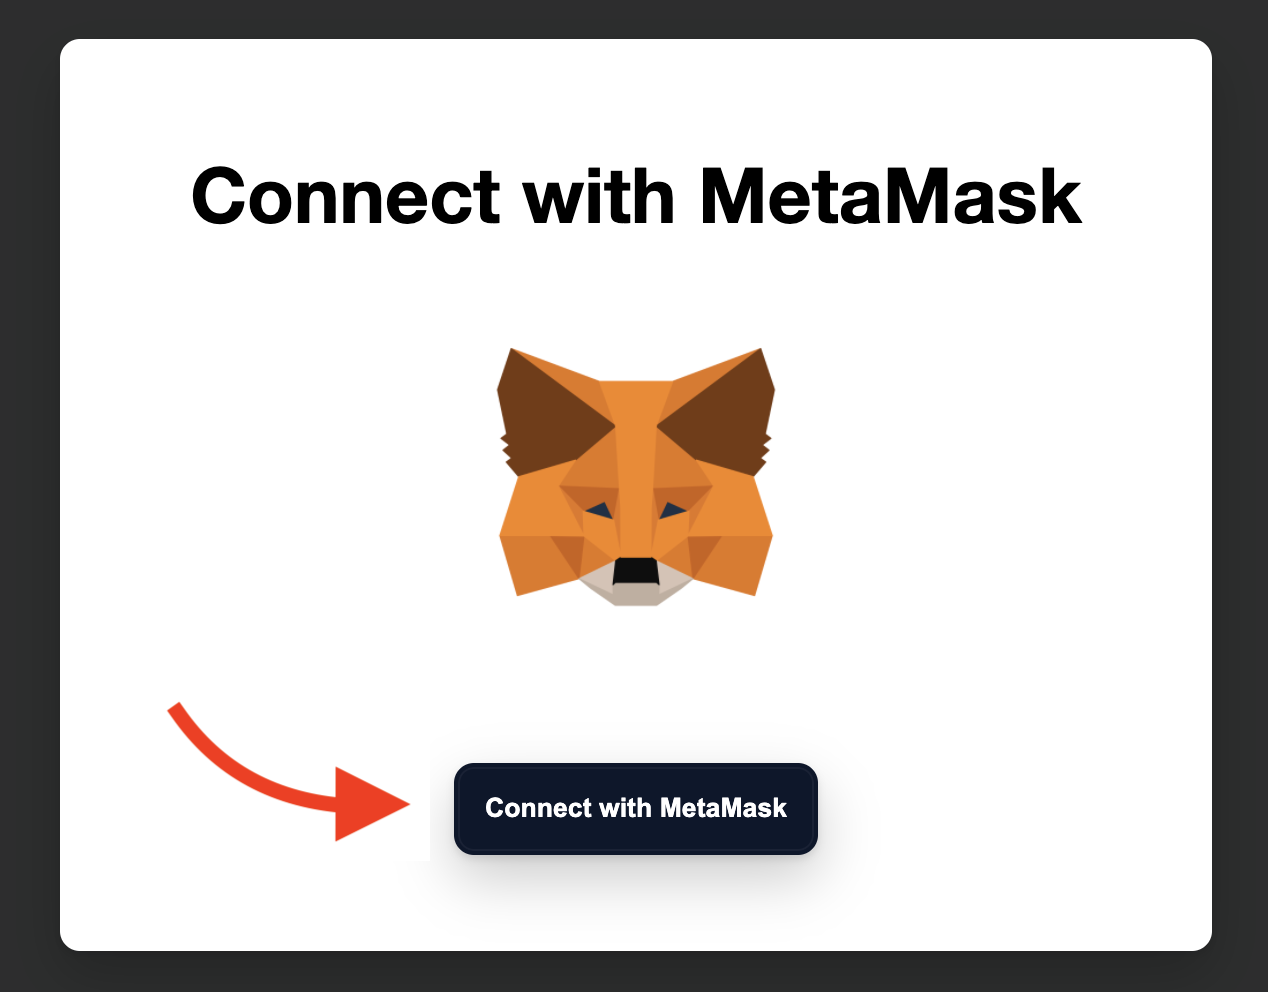
\includegraphics[width=0.5\linewidth]{img/connessione_wallet.png}
\caption{Connessione del wallet Metamask a Shop Chain.}
\end{figure}
\FloatBarrier

\section{Acquisto di un prodotto}
Per effettuare il pagamento sarà necessario detenere nel proprio wallet Metamask l'equivalente in MATIC del prezzo in dollari dell'item che si vuole acquistare. MATIC è la cryptovaluta nativa della blockchain Polygon con la quale è possibile pagare con Shop Chain.
\\É possibile scambiare le proprie cryptovalute sul network Polygon attraverso uno dei seguenti exchange decentralizzati:

\begin{itemize}
\item \href{https://www.quickswap.exchange}{QuickSwap};
\item \href{https://app.sushi.com/}{SushiSwap};
\item \href{https://polygon.curve.fi/}{Curve}.
\end{itemize}
Una volta verificato di possedere una sufficiente quantità di MATIC si può procedere col pagamento. É possibile verificare prima del pagamento l'ammontare in dollari e l'address del venditore (Fig. 2). Infine per concludere il pagamento:
\begin{itemize}
\item selezionare "Confirm" (Fig. 2);
\item confermare la transazione su Metamask.
\end{itemize}

Dovrà essere pagata anche un piccola somma per coprire i costi di transazione sul network \textit{Polygon}; questa è visualizzabile direttamente da Metamask prima di confermare la transazione.
\FloatBarrier
\begin{figure}[!h]
\centering
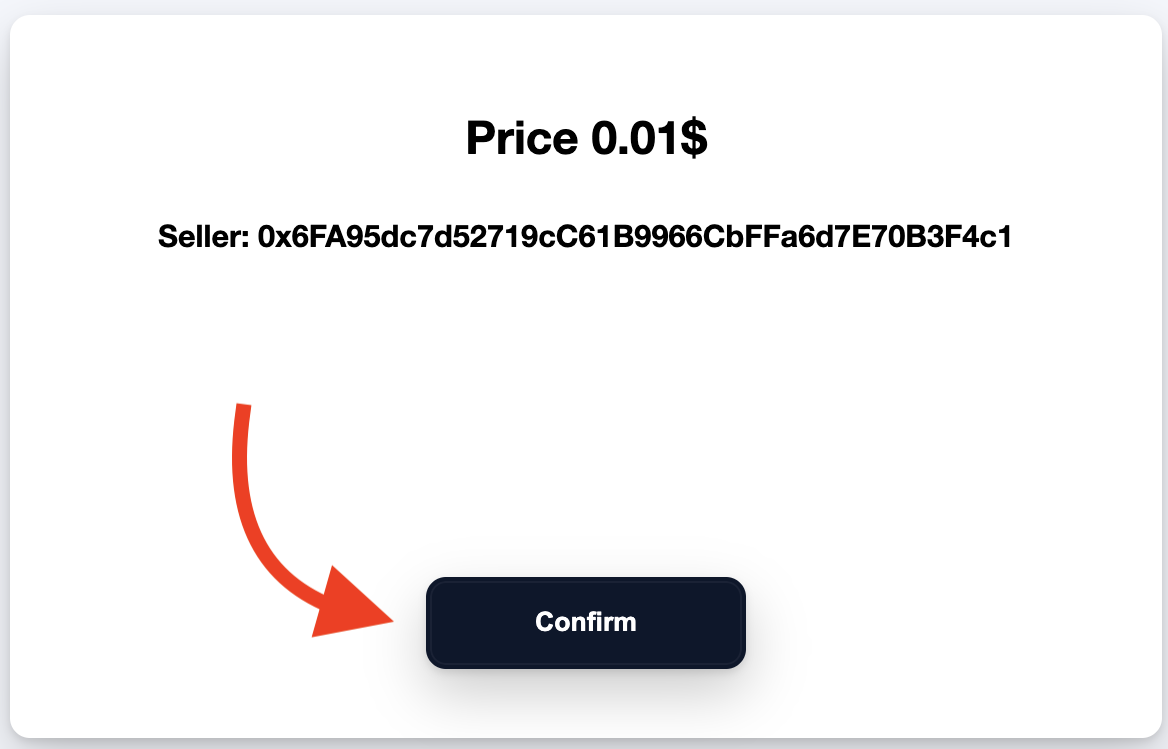
\includegraphics[width=0.5\linewidth]{img/oggetto_in_vendita.png}
\caption{Acquisto di un prodotto.}
\end{figure}
\FloatBarrier
Inoltre attraverso la sezione "Outgoing" posta nel menù in alto a destra (Fig. 3) sarà possibile visualizzare l'insieme di pagamenti effettuati con Shop Chain attraverso il wallet collegato.
\FloatBarrier
\begin{figure}[!h]
\centering
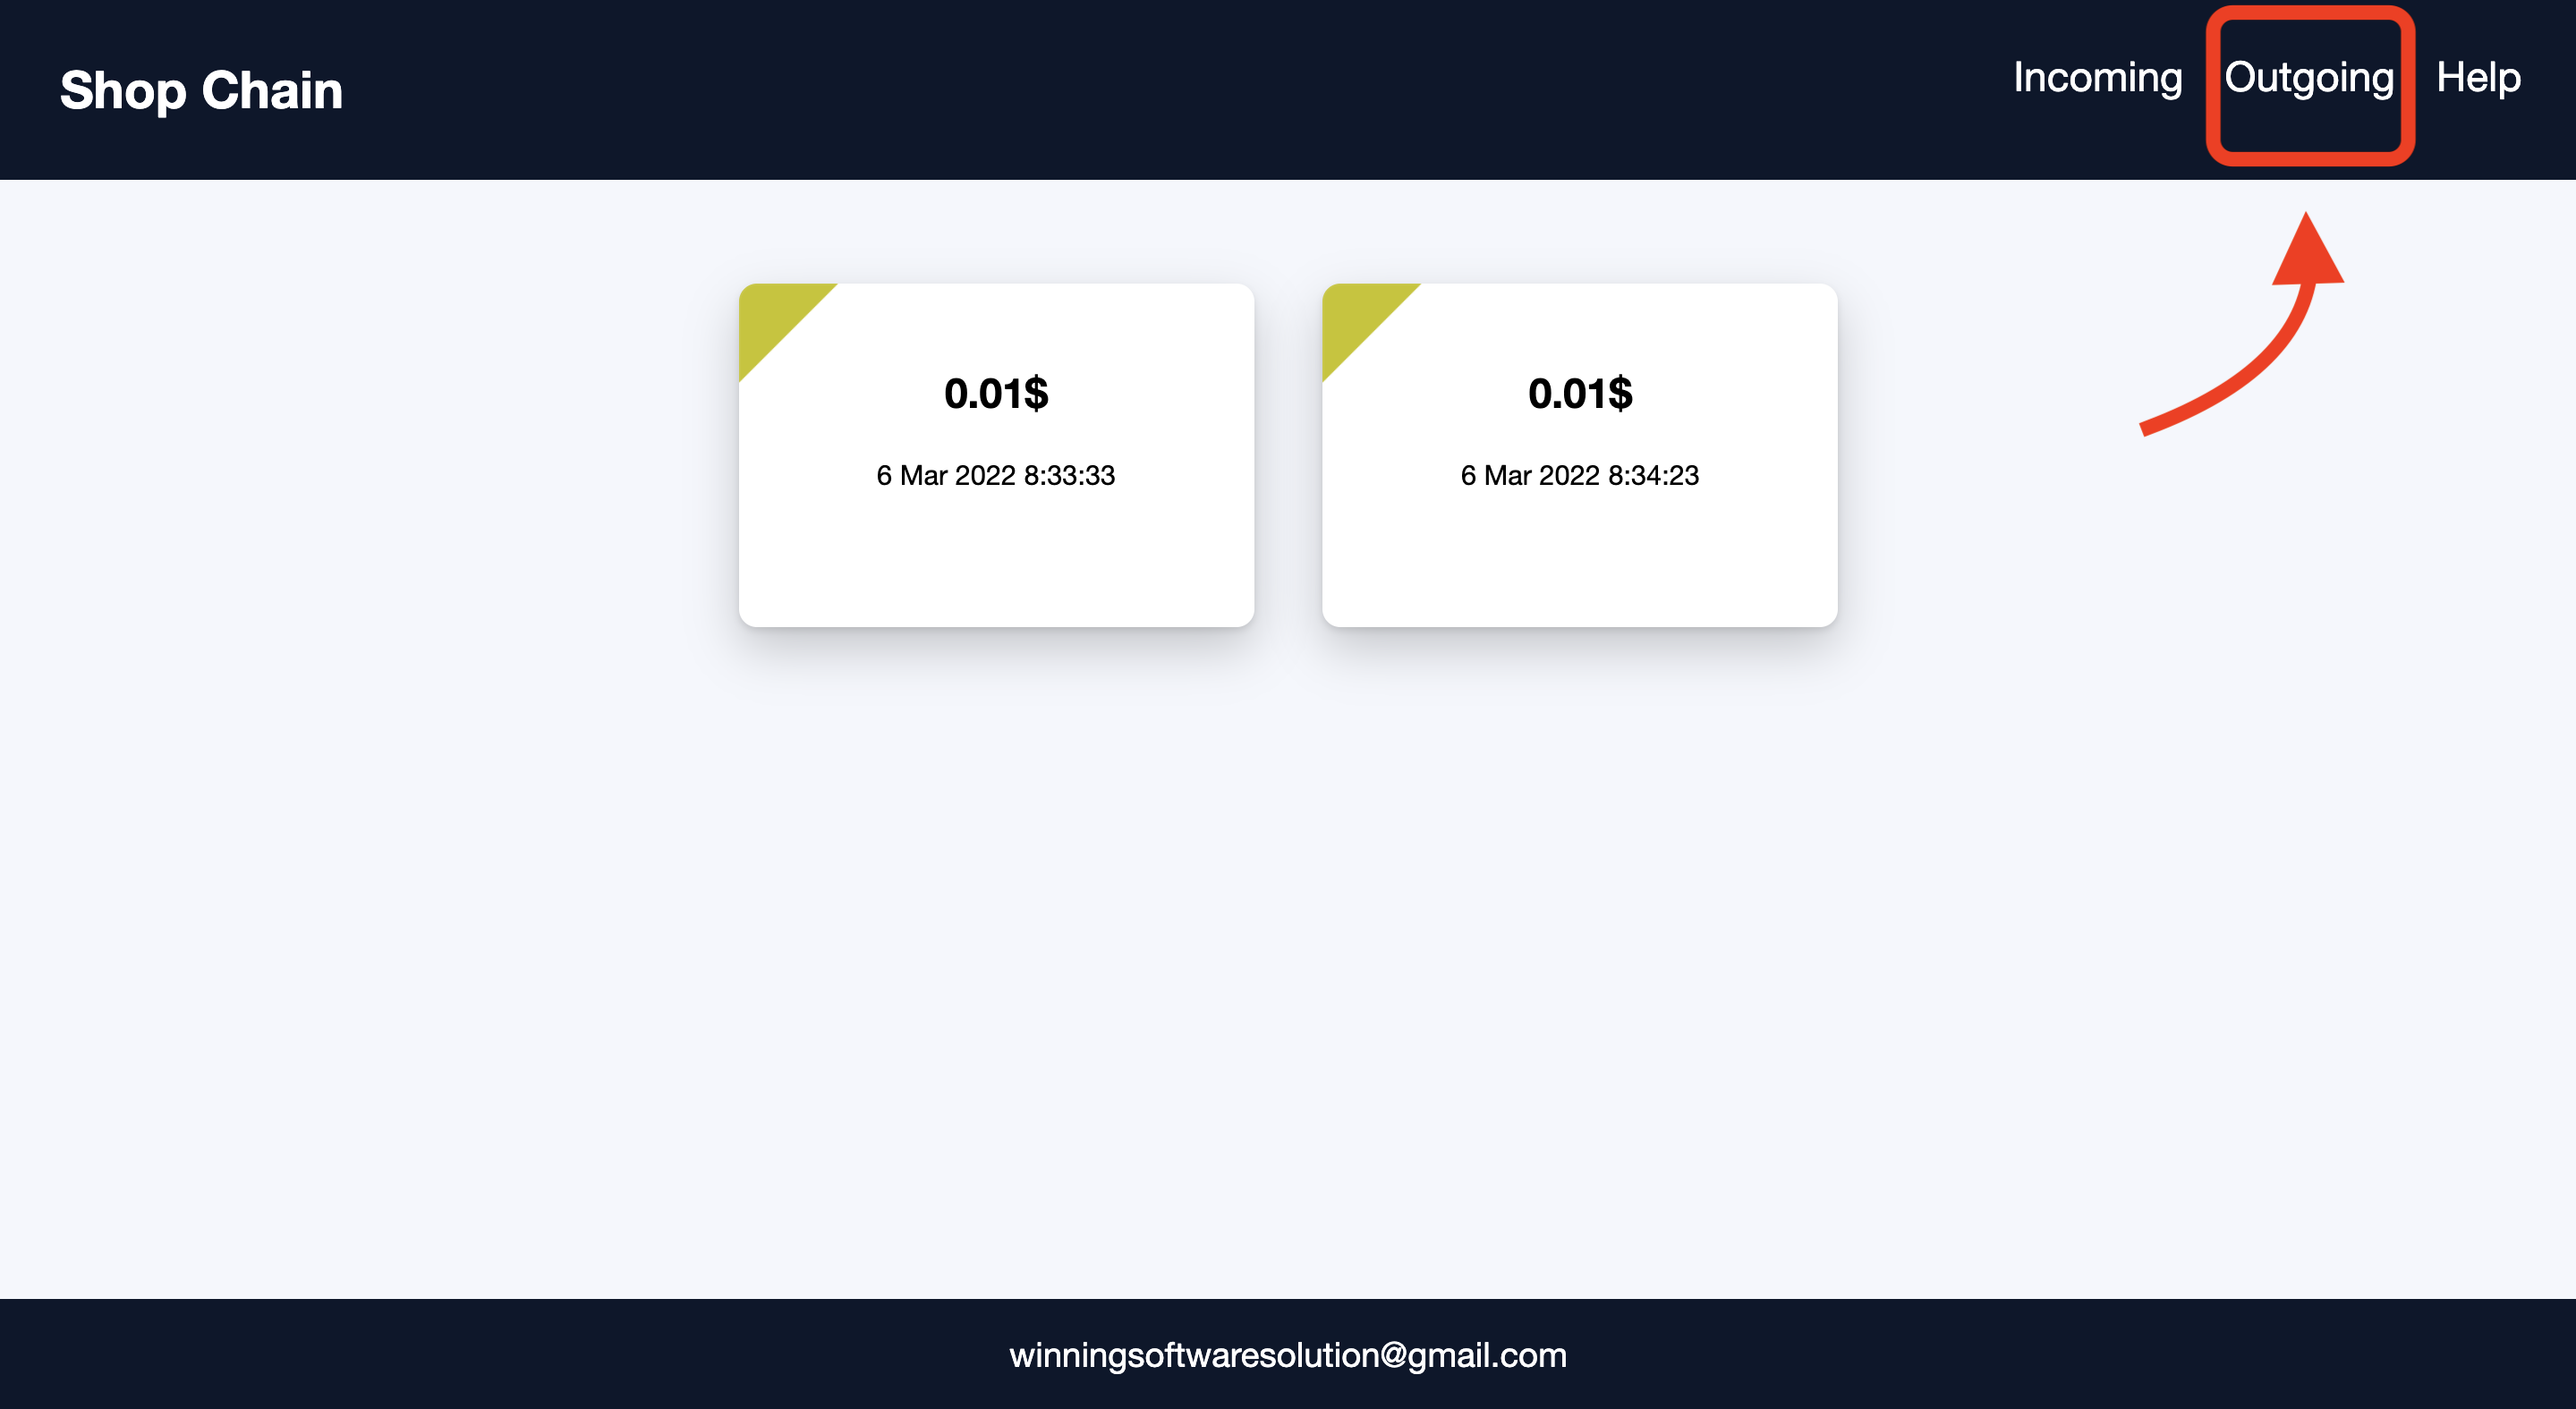
\includegraphics[width=0.8\linewidth]{img/visualizzazione_ordini.png}
\caption{Sezione Outgoing per visualizzazione pagamenti.}
\end{figure}
\FloatBarrier

\subsection{Visualizzazione acquisti}
É possibile selezionare un acquisto per visualizzare i seguenti dati (Fig. 4 riquadro 1):
\begin{itemize}
\item \textbf{Price}: indica il prezzo dell'oggetto acquistato;
\item \textbf{From}: indica l'address del wallet dal quale è stato eseguito il pagamento;
\item \textbf{To}: indica l'address del wallet del venditore;
\item \textbf{Opened}: indica la data in cui è stato eseguito l'acquisto;
\item \textbf{Expired}: indica la data in cui scade l'ordine e in cui i fondi vengono automaticamente rimborsati, si tratta di 14 giorni dopo l'acquisto.
\item \textbf{Stato dell'ordine}:
  \begin{itemize}
    \item \textbf{Open}: l'ordine è ancora aperto e in attesa di conferma;
    \item \textbf{Confirmed}: l'ordine è già stato confermato attraverso la scannerizzazione del codice QR;
    \item \textbf{Expired}: l'utente ha chiesto il rimborso poiché non ha ricevuto il pacco entro 14 giorni;
    \item \textbf{Canceled}: l'ordine è stato rifiutato dall'e-commerce. I fondi utilizzati per il pagamento vengono restituiti all'acquirente nella valuta stabile DAI.
  \end{itemize}
\end{itemize}
\subsection{Gestione acquisti}
Dopo 14 giorni dalla data di acquisto, se i fondi non sono stati sbloccati dall'acquirente attraverso la scannerizzazione del codice QR, avverrà il rimborso in DAI dell'esatto importo pagato. Nel caso in cui dopo 14 giorni l'acquirente non ha ancora ricevuto né il pacco né il rimborso, potrà annullare il pagamento manualmente selezionando l'opzione "Refund transaction" (Fig. 4 riquadro 2) e dunque ricevere il rimborso.
\FloatBarrier
\begin{figure}[!h]
\centering
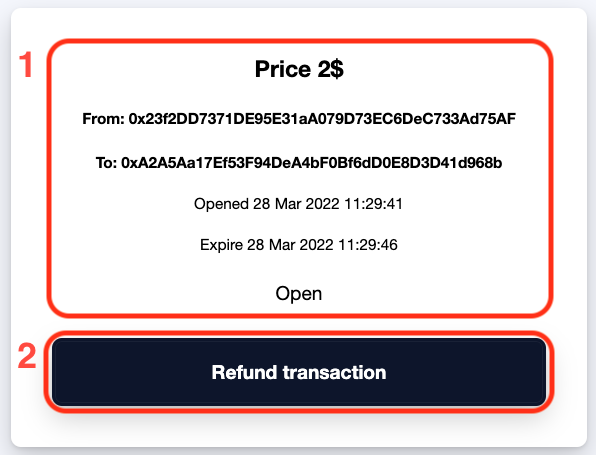
\includegraphics[width=0.8\linewidth]{img/transazione_acquirente.png}
\caption{Visualizzazione e gestione acquisti.}
\end{figure}
\FloatBarrier
\section{Sblocco dei fondi}
Per tutelare l'acquirente, i MATIC utilizzati per il pagamento sono bloccati e il venditore non può utilizzarli fino al momento della ricezione del pacco. Al momento della consegna l'acquirente deve sbloccare i fondi.\\
I seguenti paragrafi descrivono la procedura da seguire per concludere l'acquisto e sbloccare correttamente i fondi.
\subsection{Scannerizzazione codice QR}
Il venditore al momento della spedizione attacca sulla scatola un codice QR. L'acquirente, dopo il ritiro del pacco, deve procedere con la scannerizzazione di questo codice QR per poter raggiungere la pagina di sblocco dei fondi. La scannerizzazione può essere eseguita dal proprio smartphone in due modi:
\begin{itemize}
\item applicazione specifica per la scannerizzazione di codici QR: inquadrare il codice QR dalla propria fotocamera e seguire il reindirizzamento a Metamask;
\item applicazione Metamask: selezionare l'opzione di scannerizzazione internamente a Metamask.
\end{itemize}
In entrambi i casi si viene reindirizzati alla pagina Shop Chain nel browser interno di Metamask per confermare la ricezione del pacco e sbloccare i fondi.

\subsection{Conferma dell'ordine}
Prima di procedere con la conferma dell'ordine controllare di:
\begin{itemize}
\item utilizzare il network corretto come spiegato al punto \hyperref[sec:network]{2.1.1};
\item utilizzare il wallet con il quale è stato eseguito il pagamento, altrimenti non sarà possibile la conferma;
\item detenere alcuni MATIC per il pagamento delle tasse per la transazione di conferma.
\end{itemize}
Una volta reindirizzati sulla landing page per la conferma dell'acquisto è possibile controllare i dati dell'ordine. Infine procedere come segue:
\begin{itemize}
\item selezionare "Confirm" (Fig. 4);
\item confermare la transazione di conferma su Metamask.
\end{itemize}
\FloatBarrier
\begin{figure}[!h]
\centering
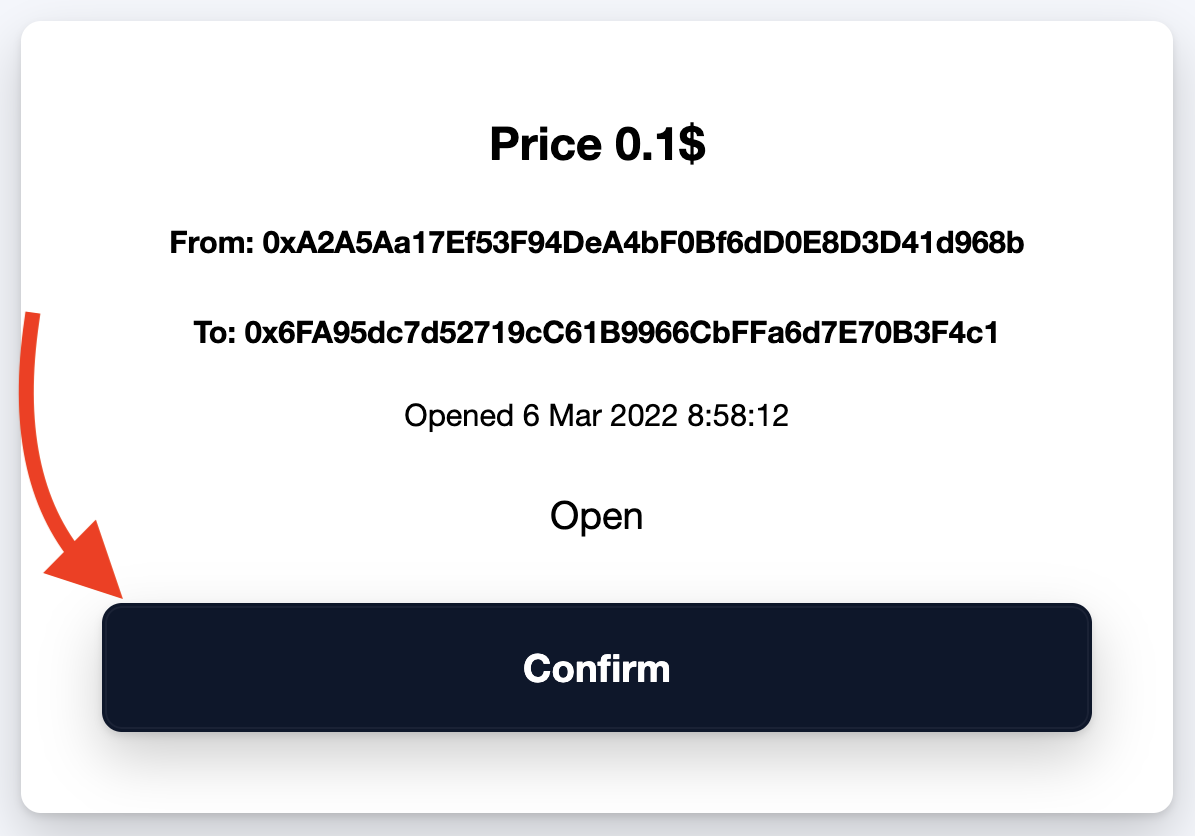
\includegraphics[width=0.5\linewidth]{img/conferma_ordine.png}
\caption{Interfaccia per la conferma dell'ordine.}
\end{figure}
\FloatBarrier
\mbox{}\\
Terminata la procedura i fondi saranno resi disponibili al venditore, lo stato dell'ordine diventa "Confirmed" e dunque il processo di vendita si è concluso correttamente.
\\ \\
Grazie per aver utilizzato Shop Chain!



\end{document}
